\section{Eigenvalue solution by Power Method on GPU}
\label{sec:ev}
The last problem concerns the evaluation of eigenvalue using the power method via a paralellized CUDA code. Reference for this implementation is a sequantial CPU-code provided by the course (\texttt{power\_cpu.cu}).\\

A scematic overview of the iteration loop for the power method is shown bellow in algorithm \autoref{alg:power_method}. The whole implementation details can be found in the appendix for the current section.\\
\begin{algorithm}
    \caption{\Shining{GPU Power Method}}
    \label{alg:power_method}
    \begin{algorithmic}[1]
    \State \textbf{Input:} Matrix $\mathbf{A}$ of size $N \times N$, tolerance $\epsilon$, maximum iterations $max\_iter$
    \State \textbf{Output:} Dominant eigenvalue $\lambda$
    
    \State Initialize $\mathbf{v}$ with $v_1 = 1, v_i = 0$ for $i > 1$
    \State $\lambda_\text{Old} \gets 0$, $\lambda \gets 0$
    \State Allocate GPU memory for $\mathbf{A}$, $\mathbf{v}$, $\mathbf{w}$, and $\lambda$
    \State Copy $\mathbf{A}$ and $\mathbf{v}$ to GPU memory
    \State $\mathbf{w} \gets \mathbf{A} \cdot \mathbf{v}$ \Comment{First iteration of $\mathbf{w}$ computation using $\texttt{Av\_Product}$ kernel}
    
    \For{$i = 0$ to $max\_iter - 1$}
        \State Compute norm of $\mathbf{w}$: $\text{norm} \gets \sqrt{\mathbf{w}^T \cdot \mathbf{w}}$ \Comment{Using $\texttt{FindNormW}$ kernel}
        \State Normalize $\mathbf{v}$: $\mathbf{v} \gets \mathbf{w} / \text{norm}$ \Comment{Using $\texttt{NormalizeW}$ kernel}
        \State Compute $\mathbf{w} \gets \mathbf{A} \cdot \mathbf{v}$ \Comment{Using $\texttt{Av\_Product}$ kernel}
        \State Compute eigenvalue: $\lambda \gets \mathbf{v}^T \cdot \mathbf{w}$ \Comment{Using $\texttt{FindNormW}$ kernel}
        \If{$|\lambda - \lambda_\text{Old}| < \epsilon$}
            \State \textbf{Break} \Comment{Convergence achieved}
        \EndIf
        \State $\lambda_\text{Old} \gets \lambda$
    \EndFor
    
    \State Copy $\lambda$ back to host memory
    \State Deallocate GPU memory
    \end{algorithmic}
\end{algorithm}

\textbf{Note:} A $sqrt()$ was added in the \texttt{NormalizeW} kernel over \texttt{g\_NormW[0]}. This way we can use the output of \texttt{FindNormW} directly in the \texttt{NormalizeW} kernel.\\


I performed all the following measurements after throwing away the first GPU run (burner-run). The reason beaing, that the first run always took around 10 times longer than the following runs. This is likely due to some GPU initialization and setup overhead. It should also be noted, that I freed the GPU memory after each run to avoid caching effects. The basic setup in the main looks like this schematically: 
\lstinputlisting[language=c]{input/code/03/gpu_main.c}
Here \texttt{RunGPUPowerMethod} runs the power method on the GPU and on the top we can see the burner run. \texttt{CleanGPU} is a function that frees the allocated memory on the GPU as mentioned above.\\

\Shining{Iterations to convergence needed}\\
While performing the different measurements on the GPU it stood out to me, that the iterations needed to reach the specified tolerance ($\epsilon = 0.000005$) varied quite a bit. It was evident, that the GPU reaches a value very close to the eigenvalue rather fast (on the second iteration). However, the final convergence seems to depend on the precision of the operations. For the CPU we always perform the same operations in the same order, thus leading to the same results every time. The GPU on the other hand perfroms the calculations in parallel and especially for the accumulation operations the order of operations will certainly vary. Small rounding error introduced by the floating point percision in combination with a small $\epsilon$ can now lead to differences: These arise because the rounding in the accumulation functions such as \texttt{FindNormW} and \texttt{ComputeLamda} is dependant on the order of operations (not associative)! It should also be noted that the T4 GPUs used on Google Colab support only FP32 operations, thus moving to FP64 wasn't an option. \\

\textbf{All of the following benchmarks are perfromed in the supplied IPython notebook on Google Collab using T4 GPUs.}\\ 

\subsection{Step 1: Shared vs. global memory for matrix-vector multiplication}
As can be seen in the code snippet from above, we perfrom multiple runs of the power method on the GPU. First with global memory and then with shared memory. This is done by using different kernels for the AV-product. The kernel used for shared memory is unchanged.
Furthermore, to investigate the performance impact of shared vs. global memory during the matrix vector multiplication we first need an alternative kernel which doesn't use shared memory. This kernel is given bellow: 
\lstinputlisting[language=c]{input/code/03/Av_Product_Global.c}
Notice that the kernel above doesn't need to copy data from global to shared memory, this makes it possible to efficiently calculate the AV-product in a striped partitioning fashing. Furthermore, we do not need any syncronisation here in contrast to the original kernel. Given this, at least from a instruction flow perspective, one may think that the global memory kernel is heavily favoured due to it's simplicity. We shall see if this holds up given our measurements. \\ 
Subsequently, 10 measurements are perfromed with the original kernel and the changed kernel to determine the mean total runtimes depending on memory usage patterns. 
We obtain a \Shining{scatter plot} seen in \autoref{fig:cuda_step1}
\begin{figure}[H]
    \centering
    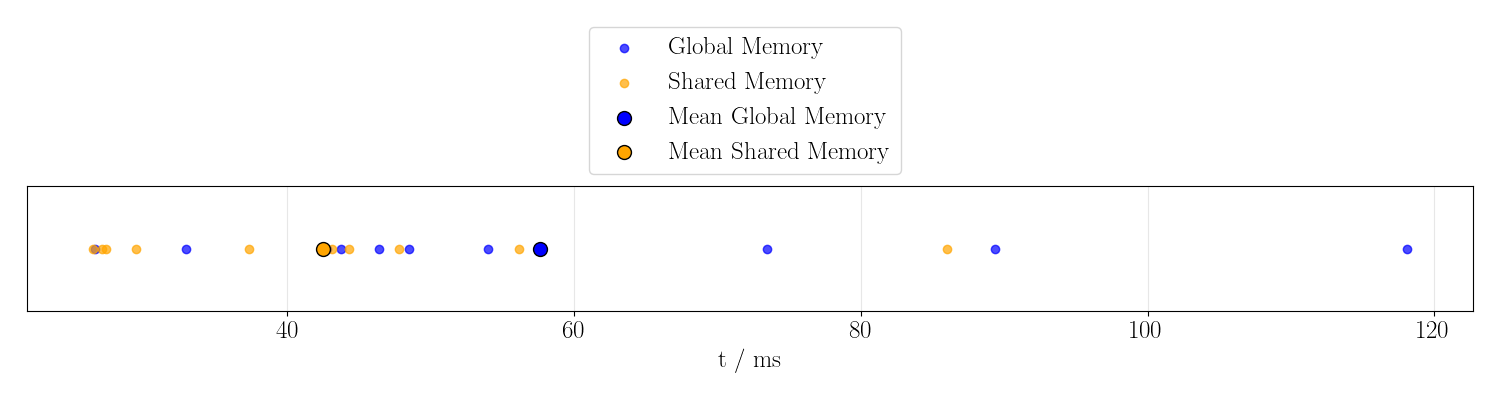
\includegraphics[width=\textwidth]{../fig/lab3/step1.png}
    \caption{Measurements }
    \label{fig:cuda_step1}
\end{figure}
Furthermore, we obtain a mean time using global memory of $t_{global} = \SI{57.6(7)}{\milli\second}$ and by using shared memory in this kernel we get $t_{shared} = \SI{42.5(3)}{\milli\second}$. 
This means we have time savings of $\SI{26(1)}{\percent}$ or about $\nicefrac{1}{4}$ when using shared memory compared to global memory. \\
\Shining{Why is shared memory faster?}\\
First and foremost we shall keep in mind, that the shared memory kernel is at a disadvantage in our comparison with the global kernel. To get insights why it still performs faster we look at benchmark results for the T4 cards to answer this question. According to a benchmark by Liu, et al. \footnote{Liu, Andy T., Yang, Shu-wen, Chi, Po-Han, Hsu, Pei-Hung, and Lee, Hung-yi. "Mockingjay: Unsupervised Speech Representation Learning with Deep Bidirectional Transformer Encoders." \textit{arXiv preprint arXiv:1903.07486}, 2019. \url{https://arxiv.org/abs/1903.07486}} not all cards have lower latency for shared memory compared to global memory. However, as their research showed the latency for the T4 architecture is actually lower by a factor of around 2-10 (depending on the number of threads simultaniously accessing the same memory bank). Additional, the bandwidth of the shared memory is much higher (> Tb/s \footnote{I sadly couldn't find information about the exact bandwidth of the shared memory}) compared to the global memory (360 Gb/s). A lower latency and higher bandwidth for the shared memory thus makes the difference. In our problem, matrix-vector multiplication, we use the matrix rows multiple time (dimensionality of vector!) and therefore the first copy operation of the data from global to shared memory pays off. \\
Stated differently, we sacrefice at first by copying to shared memory to gain better data locality and use this to our advantage in the actual calculation. 

\subsection{Step 2: Execution time for different N and threads per block}
I implemented a small loop to run the GPU code for 5 different $N$ with $N \in \{50, 500, 2000, 4000, 5000\}$. The resulting time benchmarks for 32, 64 and 100 threds per block can be seen in \autoref{fig:cuda_step2}. 
\begin{figure}[H]
    \centering
    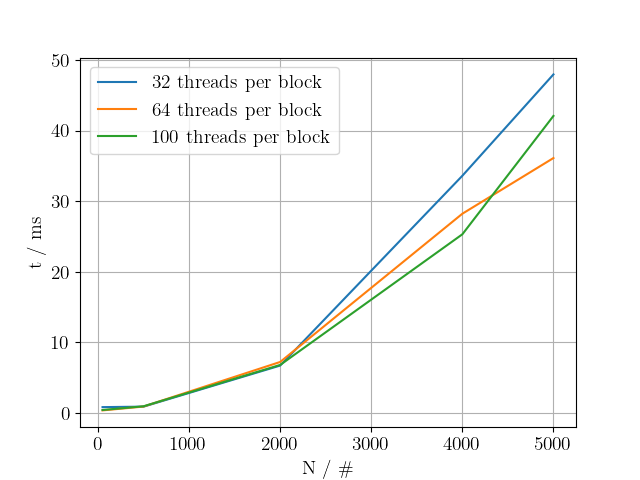
\includegraphics[width=0.5\textwidth]{../fig/lab3/step2.png}
    \caption{Runtime for $N \in \{50, 500, 2000, 4000, 5000\}$ and for 32, 64 and 100 threads per block respectively.}
    \label{fig:cuda_step2}
\end{figure}
Looking at the results we do not see an overall fastest option with 64- and 100-threads per block changing places. On the other hand, the 32- \& 96-threads per block option seem to be the slowest in terms of total runtime. \\

\Shining{Interpretation of the results}\\
The threads of a block are usually further subdivided into different wraps which perform the actual SIMT opertations. NVidia GPUs usually have a warp size of 32 threads which means for our first option (blue line in \autoref{fig:cuda_step2}) we only have one warp per block. Since warps are scheduled at the same time for the same operation (SIMT) pipelining within one wrap is not possible. However, multiple wraps in one block might be pipelined in order to hide latency. Therefore, it is plausible that for the second option (orange line in \autoref{fig:cuda_step2}) two wrap could hide some latency of each other. While one wrap is computing stuff using the ALU the other one might access memory already and vice versa. \\
Given the not so clear result between the with 64- and 100-threads case we should focus the multiplicity of 32 first. It would inherently mean that we have 4 wraps and the last has 28 (32*4 - 28 = 100) threads which lay dormant. This is generally inefficient because these threads can't do work due to the software limitation imposed.\\
Ultimately this problem is a very complex problem of latency and latency hiding and (used/unused) hardware optimization. There is no clear trend, as can be seen by the 96-threads per block option which is not really noticably better most of the time compared to the 32-threads per block option. In practice it is best to determine the most efficient thread per block size for the given problem and grid size experimentally. 


\subsection{Step 3: Speedups}
Now we really dive into the benefits of GPUs over CPUs in terms of computation speed for paralellizable programs. \\

We measure two different scenario's computation time: 
\begin{enumerate}[i]
    \item excluding time of memory copy from CPU $\rightarrow$ GPU
    \item including time of memory copy from CPU $\rightarrow$ GPU
\end{enumerate}
After measuring \Shining{5} rounds without (i) and with (ii) memory access time we obtain the following \Shining{scatter plot} in \autoref{fig:cuda_step3}. For these measurements the initial shared memory kernel was used. 
\begin{figure}[H]
    \centering
    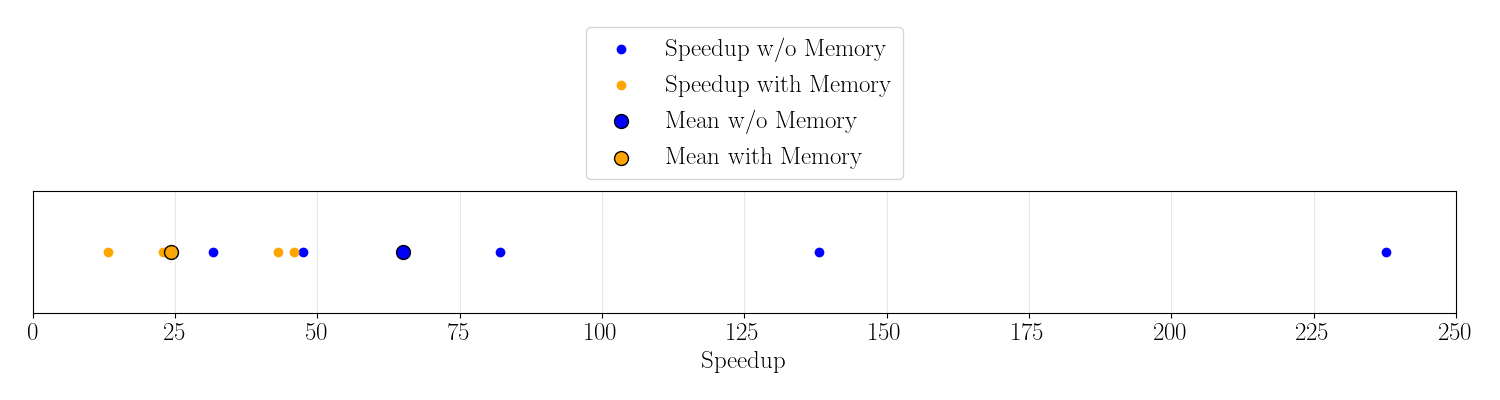
\includegraphics[width=\textwidth]{../fig/lab3/step3.png}
    \caption{Speedup of GPU implementation vs. CPU with and without memory transfer times.}
    \label{fig:cuda_step3}
\end{figure}
The mean speedup without memory access times is $\times 65$ and with memory access timed it comes out to $\times 24$.\\

\Shining{Why is there such a huge speedup when switching to GPU?}\\
As touched upon above, the SIMD/SIMT nature of GPUs let's them parallize work much more efficiently than a CPU. While it is true that a CPU could also use multiple threads\footnote{This is of course only "simulated" or software-level parallelisim since they are scheduled after one another by the OS!} or processes\footnote{This on the other hand is true parallelisim: e.g. MPI}, CPUs have way fewer cores (roughly a factor of 100) compared to GPUs. The high number of seperate Cores makes GPUs so fast because they all run simultaniously on different parts of the data.\\
A short theoretical derivation may give us more insights into the speedup we might expect from a GPU: \\
Given that a CPU (take a typical Ryzen Server CPU with 64 cores) has around 50 GFLOPS/core and a T4 GPU has 8 TFLOPS in total in single-precision. We pit them against each other (CPU without MPI -> only one core): 
\[\text{speedup}_\text{theory} = \nicefrac{8000}{50} = 160\]
We can expect a speedup of around 160 times without taking transfer time and other overhead of a GPU into account. This seems quite plausible because we indeed measure a speedup of a factor around 65. The reduction from 160 to 65 is likely due to the added complexity in memory operations $\rightarrow$ copying into shared memory and out again and setup times for the GPU kernels.  

\subsection{Step 4: Explanation of the Results}

The GPU implementation of the power method demonstrates significant performance benefits across multiple aspects. In \textbf{Step 1}, comparing global and shared memory usage, we observed a clear advantage for shared memory, with a time saving of around \( \SI{26}{\percent} \). This improvement is due to the lower latency and higher bandwidth of shared memory compared to global memory, which allows for efficient reuse of matrix rows during matrix-vector multiplication. Despite the initial cost of copying data into shared memory, the better data locality and reduced global memory accesses outweigh this overhead, leading to faster overall computation.\\

In \textbf{Step 2}, the analysis of execution time for varying numbers of threads per block highlighted the importance of optimizing thread configurations. Blocks with 64 threads performed better for the biggest problem, likely due to efficient warp utilization, allowing latency hiding between multiple warps. Blocks with 32 threads suffered from insufficient pipelining as only one warp could be active at a time, while 96- and 100-thread (for the biggest problem) configurations showed diminishing returns due to inefficiencies such as underutilized threads or increased memory contention. This emphasizes the need to experimentally determine the optimal thread count for a specific problem and grid size.\\

Finally, in \textbf{Step 3}, we observed a significant speedup of \( \times 65 \) without memory transfer times and \( \times 24 \) when including memory transfers, compared to the CPU implementation. The GPU's massively parallel architecture allows it to handle matrix-vector multiplications more efficiently than CPUs with limited cores. However, the reduction in speedup when including memory transfers reflects the overhead of data movement between CPU and GPU memory. The theoretical speedup derived from FLOPS capabilities aligns well with these results, validating the practical measurements. Variations in GPU convergence times were attributed to floating-point precision and non-associative operations, which differ from the deterministic order of operations on CPUs.\\

Overall, the results highlight the importance of leveraging GPU-specific optimizations like shared memory and optimal thread configurations while managing overheads such as memory transfers (especially form CPU to GPU and back).
